\documentclass[letterpaper, 10 pt, conference]{ieeeconf}
\IEEEoverridecommandlockouts
\overrideIEEEmargins

\let\proof\relax
\let\endproof\relax
\usepackage{amsmath,amssymb,amsfonts}
\usepackage{amsthm}
\usepackage{algorithmic}
\usepackage{algorithm}
\usepackage{graphicx}
\usepackage{graphbox}
\usepackage{textcomp}
\usepackage{multirow}
\usepackage{xcolor}
\usepackage[export]{adjustbox}
\usepackage{color}
\usepackage{hyperref}
\usepackage{pgfplots}
\usepackage{cite}

\def\BibTeX{{\rm B\kern-.05em{\sc i\kern-.025em b}\kern-.08em
    T\kern-.1667em\lower.7ex\hbox{E}\kern-.125emX}}

% Adjust table column separation if desired
\setlength{\tabcolsep}{0.4em}

\title{\LARGE\bf Runtime-Switchable Heuristics in A* for Autonomous Robots}
\author{\centering Ignacio Pastore Benaim, David Padilla Orenga}

\begin{document}
\setlength{\parskip}{0.5em} % Espacio entre párrafos
\maketitle

%%%%%%%%%%%%%%%%%%%
% ABSTRACT %
%%%%%%%%%%%%%%%%%%%
\begin{abstract}
This document presents a practical exploration of integrating a global planner based on the A* algorithm with runtime-switchable heuristics for ROS-based autonomous navigation. Traditional A* implementations utilize a fixed heuristic, which can limit adaptability across diverse environments. Our approach introduces a flexible framework that allows dynamic heuristic selection (e.g., Manhattan, Euclidean, Chebyshev) during execution without requiring navigation stack restarts.

We demonstrate the methodology, implementation, and experimental results obtained across various map scenarios. Experiments highlight how adaptive heuristic switching can improve planning times and path quality by tailoring the heuristic to specific map topologies. This innovation ensures robust performance in heterogeneous environments, making it a valuable tool for autonomous robotic navigation.
\end{abstract}

%%%%%%%%%%%%%%%%           
% INTRODUCTION %
%%%%%%%%%%%%%%%%
\section{Introduction}\label{sec:intro}

In autonomous robotics, global path planning is critical for navigating complex environments. 
Algorithms such as Dijkstra, A*, and RRT* have become foundational tools, with A* standing out due to 
its balance between optimality and computational efficiency. Introduced by Hart, Nilsson, and Raphael in
 their seminal work \cite{hart1968formal}, the A* algorithm combines the advantages of Dijkstra's 
 algorithm and greedy best-first search by using a heuristic function to estimate the cost to the goal, 
 ensuring both optimality and completeness when the heuristic is admissible.

Despite its effectiveness, traditional A* implementations rely on a fixed heuristic function, such as Manhattan (L1 norm) or Euclidean (L2 norm), which can constrain performance in dynamic or heterogeneous environments. Different heuristics have varying strengths; for example, Manhattan is well-suited for grid-based maps with axis-aligned obstacles, while Euclidean provides better results in open spaces. However, a static heuristic limits the algorithm's ability to adapt to changing conditions.

This project addresses these limitations by introducing a runtime-switchable A* planner that enables dynamic heuristic selection during navigation. This feature enhances adaptability and efficiency without requiring the navigation stack to restart, making it particularly suitable for ROS-based systems.

\subsection{Project Motivation and Scope}
The primary motivation is to demonstrate the impact of heuristic selection on planning speed and path quality in grid-based navigation. The scope of this work includes developing a ROS plugin that integrates with the \texttt{move\_base} framework and supports dynamic heuristic switching. Key components include:
\begin{itemize}
	\item The ROS Navigation Stack for costmap generation and path execution,
	\item A custom global planner plugin implementing A*,
	\item Dynamic Reconfigure for runtime heuristic adjustments.
\end{itemize}

\subsection{Literature Review}
Recent studies underscore the importance of heuristic selection in grid-based path planning. For instance, Manhattan (L1 norm) excels in structured, corridor-like environments, while Euclidean (L2 norm) is more effective in open spaces \cite{thrun2005probabilistic, lavalle2006planning}. Advanced methods such as RRT* \cite{karaman2011sampling} provide smooth paths but at a higher computational cost. This work builds on the foundational insights of Hart et al. \cite{hart1968formal}, emphasizing the flexibility of A* through heuristic switching to address these challenges.

\subsection{Outline of Approach}
The remainder of this paper is organized as follows:
\begin{itemize}
	\item Section~\ref{sec:method} details the classical A* algorithm and our modifications for heuristic switching.
	\item Section~\ref{sec:implementation} describes the ROS plugin architecture and implementation.
	\item Section~\ref{sec:experiments} presents experimental results on various map types.
	\item Section~\ref{sec:conclusion} concludes with key findings and future research directions.
\end{itemize}


%%%%%%%%%%%%%%%%%%%%%%%%           
%%% METHOD %%%
%%%%%%%%%%%%%%%%%%%%%%%%
\section{Method Description}\label{sec:method}
A* \cite{hart1968formal} is a graph-based path planning algorithm that expands 
nodes from a start position until reaching the goal. The priority of exploration 
is determined by:
\begin{equation}
f(n) = g(n) + h(n),
\end{equation}
where $g(n)$ is the cost from the start to node $n$ and $h(n)$ is a heuristic 
function estimating the cost from $n$ to the goal. 

Common heuristic functions in 2D grids:
\begin{itemize}
    \item \textbf{Manhattan:} $h(n) = |x_{goal} - x_n| + |y_{goal} - y_n|$,
    \item \textbf{Euclidean:} $h(n) = \sqrt{(x_{goal}-x_n)^2 + (y_{goal}-y_n)^2}$,
    \item \textbf{Chebyshev:} $h(n) = \max(|x_{goal} - x_n|,\; |y_{goal} - y_n|).$
\end{itemize}

\subsection{Proposed Improvement: Runtime-Switchable Heuristic}
Rather than fix one heuristic, we introduce an interface that can \textit{toggle} 
the heuristic type (Manhattan, Euclidean, Chebyshev) at runtime. This is accomplished 
through a Dynamic Reconfigure server in ROS, enabling quick adaptation to different 
map characteristics.

%%%%%%%%%%%%%%%%%%%%%%%%           
%%% IMPLEMENTATION %%%
%%%%%%%%%%%%%%%%%%%%%%%%


\section{Implementation}\label{sec:implementation}

\subsection{System Overview}
Our approach provides a plugin that implements the \texttt{nav\_core::BaseGlobalPlanner} interface, making it compatible with the standard ROS Navigation Stack (\texttt{move\_base}). Specifically, this plugin is declared as:

\begin{itemize}
    \item \textbf{Heuristics4AStar (Plugin):} A library that extends \texttt{nav\_core::BaseGlobalPlanner} and implements A* with runtime-switchable heuristics, along with a Dijkstra fallback.
    \item \textbf{Costmap2DROS:} Provides obstacle/costmap data from sensor inputs; used by the planner to determine feasible paths.
    \item \textbf{Dynamic Reconfigure Server:} Exposes the parameter \texttt{/GlobalPlanner/heuristic\_type} for at-runtime switching among Manhattan, Euclidean, or Chebyshev heuristics.
\end{itemize}

\subsection{Plugin Architecture}
Because the plugin inherits from \texttt{nav\_core::BaseGlobalPlanner}, it integrates seamlessly with \texttt{move\_base}. Internally, we adapt functionality from the standard \texttt{global\_planner} package (e.g., expansions, cost computations) but add our own code to handle heuristic switching via Dynamic Reconfigure. 
This design allows the \texttt{move\_base} node to recognize our planner as a valid global planner plugin and load it within the navigation configuration showed in
Figure~\ref{fig:rqt_graph}.

Hence, from the perspective of the navigation stack, our planner is loaded dynamically at runtime as \texttt{heuristics4astar/GlobalPlanner}.

\begin{figure}[!ht]
    \centering
    % Placeholder for your rqt_graph or similar
    \fbox{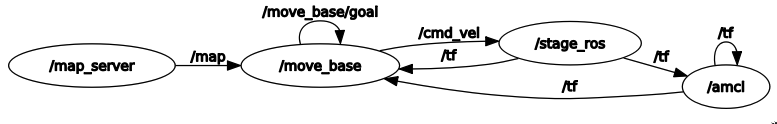
\includegraphics[width=0.90\columnwidth]{images/rqt_graph.png}}
    \caption{Conceptual Node Diagram: the custom global planner node 
    with connections to costmap and move\_base.}
    \label{fig:rqt_graph}
\end{figure}

\subsection{Key Modifications}
\textbf{Motivation:} 
Different map structures benefit from different heuristics.  
\textbf{Deviation from Standard A*}: 
We add a callback in the A* plugin that updates the “heuristic\_type” string 
(or integer) at runtime. If a user chooses a suboptimal heuristic for a large open map, planning might 
be slower. But if they switch to a more direct Euclidean measure, path length 
and timing might improve.

\begin{algorithm}[H]
\caption{Pseudo-code for Switchable A* Heuristic}
\label{alg:alg2}
\begin{algorithmic}[1]
\REQUIRE heuristic\_type in \{Manhattan, Euclidean, Chebyshev\}
\IF{heuristic\_type == Manhattan}
    \STATE $h(n) \leftarrow |x_{goal} - x_n| + |y_{goal} - y_n|$
\ELSIF{heuristic\_type == Euclidean}
    \STATE $h(n) \leftarrow \sqrt{(x_{goal}-x_n)^2 + (y_{goal}-y_n)^2}$
\ELSIF{heuristic\_type == Chebyshev}
    \STATE $h(n) \leftarrow \max(|x_{goal}-x_n|,|y_{goal}-y_n|)$
\ENDIF
\RETURN $f(n) = g(n) + h(n)$
\end{algorithmic}
\end{algorithm}


%%%%%%%%%%%%%%%           
% Experimental results %
%%%%%%%%%%%%%%%
\section{Experimental Results}\label{sec:experiments}
\subsection{Setup}
We evaluated the planner in ROS Noetic, using:
\begin{itemize}
    \item \textbf{Simulator:} Gazebo/Stage
    \item \textbf{Maps:} 
    \begin{itemize}
        \item \textbf{maze\_corridor:} A corridor-like environment with multiple turns
        \item \textbf{blank:} Very open space, minimal obstacles
        \item \textbf{corridor:} A partially blocked map with line-shaped obstacles
    \end{itemize}
    \item \textbf{Metrics:} Planning time, path length, and sum of turns
    \item \textbf{Heuristics Tested:} Manhattan, Euclidean, Chebyshev
\end{itemize}

\paragraph*{Metrics}
\textbf{Planning Time} (seconds) measures how long the global planner takes to compute a path once a new goal is received. Lower times indicate faster performance in finding a feasible route. 

\textbf{Path Length} (meters) is the total distance from start to goal, summed over all consecutive waypoints in the final plan. Shorter lengths often signify more direct or efficient routes in terms of travel distance.

\textbf{Sum of Turns} (radians) is a proxy for \textit{smoothness}: we sum the absolute angle differences between successive segments of the planned path. A higher value indicates many sharp turns or zig-zag patterns, while lower values suggest a smoother or more continuous trajectory. Although it does not enforce dynamic constraints, this turn metric helps compare how different heuristics yield straighter or more corner-heavy paths.


\subsection{Data and Observations}
We collected 3 runs for each map and heuristic, then aggregated the results to produce mean values of time, path length, and turning cost. Table~\ref{table:aggregated} shows a summary of the computed averages for each (Map, Heuristic) combination:

\begin{table}[!ht]
\centering
\footnotesize
\caption{Aggregated Averages over Runs (Time in seconds, Length in meters, Turns in sum of turn angles).}
\label{table:aggregated}
\begin{tabular}{|l|l|c|c|c|}
\hline
\textbf{Map} & \textbf{Heuristic} & \textbf{AvgTime} & \textbf{AvgLength} & \textbf{AvgSumTurns} \\
\hline
\texttt{maze\_corridor} & manhattan & 0.0571 & 37.5759 & 324.41 \\
\texttt{maze\_corridor} & euclidean & 0.0504 & 35.0652 & 57.1588 \\
\texttt{maze\_corridor} & chebyshev & 0.0520 & 35.5563 & 56.8049 \\
\hline
\texttt{blank} & manhattan & 0.00454 & 17.2552 & 3.52737 \\
\texttt{blank} & euclidean & 0.05271 & 17.1446 & 189.8077 \\
\texttt{blank} & chebyshev & 0.07646 & 17.3730 & 195.2520 \\
\hline
\texttt{corridor} & manhattan & 0.00578 & 21.5848 & 24.8970 \\
\texttt{corridor} & euclidean & 0.03303 & 20.7376 & 31.9885 \\
\texttt{corridor} & chebyshev & 0.04731 & 21.2848 & 64.44 \\
\hline
\end{tabular}
\end{table}


\subsubsection{Qualitative Analysis per Map}
\begin{itemize}
    \item \textbf{Maze-like map (maze\_corridor)}:
    \begin{itemize}
        \item Paths bend around walls. Manhattan often takes a more “grid-aligned” route, while Euclidean and Chebyshev produce slightly smoother curves yet similar planning times.
        \item Comparing results: Manhattan is \emph{slower in planning time} and yields a \emph{much higher turn sum} than Euclidean or Chebyshev. Euclidean and Chebyshev are quite close in planning time, but Chebyshev’s path is slightly longer or differs in turn cost.
    \end{itemize}

    \item \textbf{Blank map}:
    \begin{itemize}
        \item The path is basically a straight line from start to goal under any heuristic, but \emph{Manhattan expansions are extremely fast} (about 0.0045 s). Path length is around 17.25, with only ~3.53 turns.
        \item Euclidean and Chebyshev times are higher, and they produce significantly bigger turn sums—likely because the expansions in open space allow diagonal expansions (or full expansions) that lead to more angle changes or expansions in the search.
    \end{itemize}

    \item \textbf{Corridor map (partially blocked, lined obstacles)}:
    \begin{itemize}
        \item Manhattan often yields a step-like or more direct route, while Euclidean/Chebyshev can find diagonal segments. Obstacles force detours, causing the path to weave among blocks.
        \item Manhattan is very quick again, with moderate turn sum (~24.90). Euclidean is a bit slower (0.0330 s) with ~31.99 turns. Chebyshev is intermediate in time but has a large turn sum (~64.44), suggesting more zig-zag expansions.
    \end{itemize}
\end{itemize}

\subsubsection{Visual Examples}
Figure~\ref{fig:maze_paths} showcases the path in a maze‐type environment, while Figure~\ref{fig:blank_paths} shows the nearly straight diagonal 
route in an open map, and Figure~\ref{fig:lined_corridor_paths} illustrates the corridor or lined‐obstacle scenario.
 The green lines represent the global path from the start (bottom-left) to the goal (top-right).

\begin{figure}[!ht]
    \centering
    \fbox{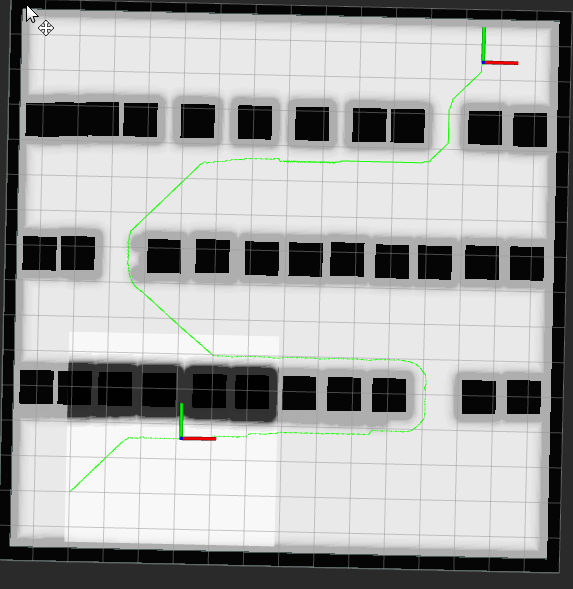
\includegraphics[width=0.8\columnwidth]{images/manhattan_maze_corridor.png}}
    \caption{Maze corridor example for manhattan heuristic taking a grid-aligned path.}
    \label{fig:maze_paths}
\end{figure}

\begin{figure}[!ht]
    \centering
    \fbox{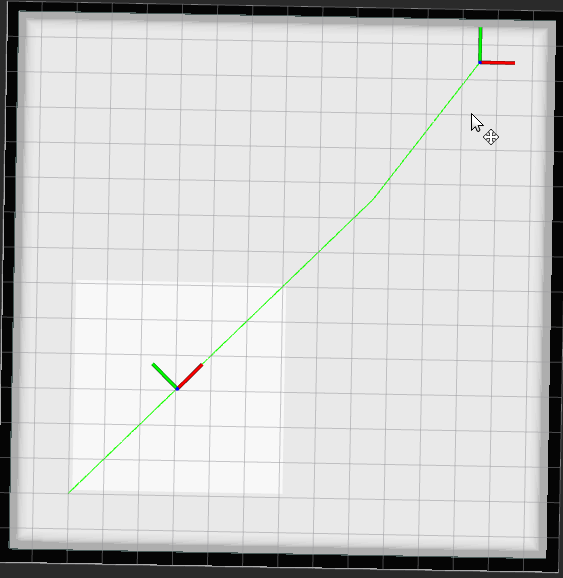
\includegraphics[width=0.8\columnwidth]{images/euclidean_blank.png}}
    \caption{Blank map example with euclidean heurisic. Almost a direct diagonal path.}
    \label{fig:blank_paths}
\end{figure}

\begin{figure}[!ht]
    \centering
    \fbox{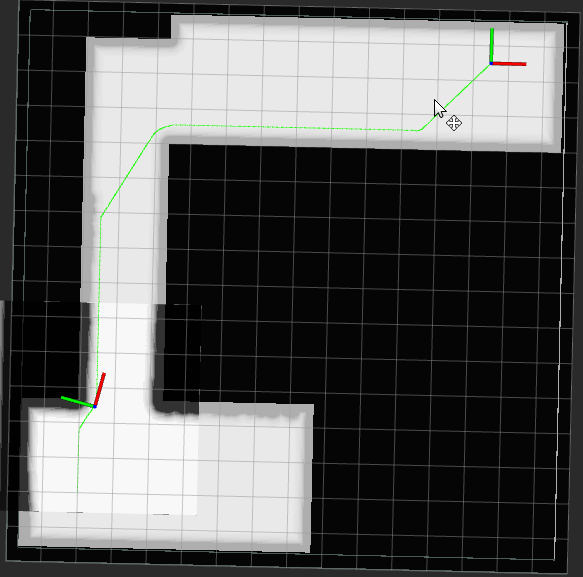
\includegraphics[width=0.8\columnwidth]{images/chebyshev_corridor.png}}
    \caption{Lined obstacles corridor example with chebyshev heuristic. The path weaves around blocks.}
    \label{fig:lined_corridor_paths}
\end{figure}

\subsubsection{Overall Conclusions from Data}
\begin{itemize}
    \item No single heuristic dominates across all maps.
    \item \emph{Manhattan} tends to be extremely fast in open spaces (\texttt{blank} map), but can produce more corners (hence a higher turn sum) in corridor-like scenarios.
    \item \emph{Euclidean} and \emph{Chebyshev} often generate more diagonal or smoother expansions, especially in partially open areas, but can show slightly longer times in simple open spaces if the expansions are large.
\end{itemize}


%%%%%%%%%%%%%%%           
% CONCLUSIONS %
%%%%%%%%%%%%%%%
\section{Conclusion and Future Work}\label{sec:conclusion}
We introduced a runtime-switchable heuristic A* planner within the ROS Navigation Stack, enabling dynamic changes among Manhattan, Euclidean, and Chebyshev heuristics at runtime. 

\textbf{Key Observations}:
\begin{itemize}
    \item \textbf{Maze-like environments}: Manhattan gave higher turn counts and was slower 
    in some runs, while Euclidean/Chebyshev remained relatively efficient with fewer sharp angles.
    \item \textbf{Open spaces}: Manhattan expansions finished extremely quickly, though path length 
    and sum of turns were very low. Euclidean/Chebyshev had more expansions and angle changes, raising turn metrics.
    \item \textbf{Corridor or lined obstacles}: Manhattan found step-like paths with moderate turn sums, 
    while Euclidean or Chebyshev sometimes introduced diagonal arcs but also occasionally higher expansions and turn sums.
\end{itemize}

\textbf{Limitations}: We tested in simulation with static obstacles; real-world trials may differ due to sensor noise and dynamic obstacles. We also did not integrate 
advanced local planners or post-processing for smoothing.  

\textbf{Future Work}: 
\begin{itemize}
    \item Evaluate the plugin on a physical robot to assess real-time performance and sensor impacts.
    \item Investigate automatic heuristic selection based on live map analysis (e.g., detecting corridor vs. open areas).
    \item Integrate advanced local planners (like TEB) or smoothing to reduce sharp path corners.
\end{itemize}

\bibliographystyle{IEEEtran}
% \bibliography{biblio}

\begin{thebibliography}{1}

\bibitem{hart1968formal} P. E. Hart, N. J. Nilsson, and B. Raphael, "A Formal Basis for the Heuristic Determination of Minimum Cost Paths," \textit{IEEE Trans. on Systems Science and Cybernetics}, vol. 4, no. 2, pp. 100--107, 1968.

\bibitem{thrun2005probabilistic} S. Thrun, W. Burgard, and D. Fox, \textit{Probabilistic Robotics}, MIT Press, 2005.

\bibitem{lavalle2006planning} S. M. LaValle, \textit{Planning Algorithms}, Cambridge University Press, 2006.

\bibitem{karaman2011sampling} S. Karaman and E. Frazzoli, "Sampling-based Algorithms for Optimal Motion Planning," \textit{The International Journal of Robotics Research}, vol. 30, no. 7, pp. 846--894, 2011.

\end{thebibliography}

\end{document}